\documentclass[12pt,twoside,a4paper]{book}
\usepackage[utf8]{inputenc}
\usepackage{tikz}
\usetikzlibrary{shapes.geometric, arrows, backgrounds, fit, decorations.pathreplacing, mindmap,trees}
\usepackage[shortlabels]{enumitem}

\newcommand{\SketchObject}{\emph{SketchObject}}
\newcommand{\Sketch}{\emph{Sketch}}

\newcommand{\textoverline}[1]{$\overline{\mbox{#1}}$}

\newenvironment{tolerant}[1]{%
  \par\tolerance=#1\relax
}{%
  \par
}

\newenvironment{dedication}
  {\clearpage           % we want a new page
   \thispagestyle{empty}% no header and footer
   \vspace*{\stretch{1}}% some space at the top
   \itshape             % the text is in italics
   \raggedleft          % flush to the right margin
  }
  {\par % end the paragraph
   \vspace{\stretch{3}} % space at bottom is three times that at the top
   \clearpage           % finish off the page
  }

\usepackage[most]{tcolorbox}
\definecolor{block-gray}{gray}{0.85}

\newtcolorbox{codequote}{colback=block-gray,grow to right by=-10mm,grow to left by=-10mm,
boxrule=0pt,boxsep=0pt,breakable}




\title{FreeCAD Sketcher Solver Architecture}
\author{Abdullah Tahiri}
\date{December 2018}


\begin{document}
    % Flow Chart nodes definitions and Styles
    \tikzstyle{startstop} = [rectangle, rounded corners, minimum width=3cm, minimum height=1cm,text centered, draw=black, fill=red!30]

    \tikzstyle{io} = [trapezium, trapezium left angle=70, trapezium right angle=110, minimum width=3cm, minimum height=1cm, text centered, draw=black, fill=blue!30]

    %\tikzstyle{process} = [rectangle, minimum width=3cm, minimum height=1cm, text centered, draw=black, fill=orange!30]

    \tikzstyle{process} = [rectangle, minimum width=3cm, minimum height=1cm, text centered, text width=3cm, draw=black, fill=orange!30]

    \tikzstyle{decision} = [diamond, minimum width=3cm, minimum height=1cm, text centered, draw=black, fill=green!30]

    \tikzstyle{surround} = [fill=blue!10,thick,draw=black,rounded corners=2mm]

    \tikzstyle{arrow} = [thick,->,>=stealth]
    % Tikz end

    \frontmatter

    \maketitle

    \begin{dedication}
        To the FreeCAD Community
        \par   %% or a blank line
        \vspace{2\baselineskip}
        To Werner for reviewing tons of lines of code per year
    \end{dedication}


    \chapter{Preface}

    Every year there are a couple of inquiries about how to get introduced into the solver code base. Motivated people with great ideas but limited time generally end up succumbing to the rather big entry energy required to understand how it is implemented.

    It is not difficult for me to understand them. I have been myself overwhelmed by it. I am still. I have been though lucky enough of having several ingredients that have allowed me to reach a certain degree of understanding of what is going on: a) motivation to undertake changes, b) support from people with a better geometry knowledge and better mathematical background, c) time.

    This document attempts to lower the entry point towards the code base of the solver.

    It is my belief that only through a diversity of opinions and ideas we can actually collaborate into making significant and meaningful improvements.

    This document should serve to gain a general common understanding allowing to identify improvements and enabling a discussion. For the rest, you are not alone. Make an account in the FreeCAD Community forum if you don't have already one. It is there that true collaboration starts.



    \tableofcontents
    \newpage

    \mainmatter

    \chapter{Introduction}

    This document is an introduction to solver architecture behind FreeCAD. It describes mainly the architecture and implementation of the solver. Other parts of the Sketcher are discussed only insofar as to enable to understand the former.

    In order to save time to most readers, let's first describe what this is not. This document is not about how to use the Sketcher to draw a shape. This document is not about how to efficiently use the Sketcher. This document is not about general Sketcher programming.

    This document tries to throw some light into how the solver actually works, and other than out of mere curiosity, it may be of little to no interest for 99.\textoverline{9}\% of the people. If you are still reading maybe you belong to that minority who is trying to:

    \begin{enumerate}[a)]
    \item Introduce support for a new geometry in the Sketcher.
    \item Introduce support for a new constraint in the Sketcher.
    \item Try to solve a bug in the solver.
    \item Get more information from the solver process to the user.
    \item Introduce a new algorithm to the solver.
    \item Improve an algorithm of the solver.
    \end{enumerate}

    You will certainly get more information than you actually need for the first two items and you will still need much more information from elsewhere. You may want to search for the git commits when the support for Hyperbola and Parabola was introduced for more information.

    For the next two items it should give you a fair overview of how things work. But it is probably for the last two items where this information may be specially valuable.

    \chapter{Sketcher Architecture}

    \section{Sketcher, solver and interface}

    A sketcher object, class \SketchObject{}, contains all the geometry and constraints that define a given Sketch, as well as all the high level functions that can be applied to a sketch to add, delete or otherwise modify this geometry.

    However, the sketcher object relies on specialised code, a geometric contraint system called PlaneGCS, in order to perform the actual solving of the constraints, which causes the geometry to adapt to those constraints.

    \begin{tolerant}{500}
    The most important concept at this architectural level is to understand that PlaneGCS does \underline{not} understand the concept of geometry and constraints used in the Sketcher. For the programmer, it is not aware of what Part::Geometry and Sketcher::Constraint are.
    \end{tolerant}

    Though this may initially seem as a design flaw or limitation, it is not. Those higher level representations of reality are very important for the remaining operations of the Sketcher, but they are useless when talking about the number of degrees of freedom introduced by a geometric shape, or to calculate the gradients to decide in which direction to move an element when seeking convergence. Similarly, the information used during solving is mostly useless at a higher level. Of course it could have been decided to put everything together, but there would be no advantages and a lot of flexibility would have been lost, for example, the ability of change to another better solver implementation if one ever is created, or to use PlaneGCS in other products (yes there are other products aside from FreeCAD that use PlaneGCS).

    \begin{figure}
    \caption{Sketcher/solver basic architecture}
    \begin{tikzpicture}[node distance=4cm]
        \node (start) [process] {Geometry \\ Constraints};
        \node (pro1) [process, right of=start] {solver interface\\ (Sketch)};
        \node (stop) [process, right of=pro1] {Solver\\(PlaneGCS)};
        \draw [arrow] (start) -- (pro1);
        \draw [arrow] (pro1) -- (stop);
        \begin{pgfonlayer}{background}
            \node[inner xsep=10pt, inner ysep=10mm, surround] (background) [fit = (start) (stop) (pro1)] {};
            % label
            \node[above left] at (background.south east) {SketchObject};
        \end{pgfonlayer}
    \end{tikzpicture}
    \end{figure}

    Having a higher level Sketcher that understands a representation of the geometry and a solver that uses a different one, makes necessary to bring an interface therebetween in order to connect both. This interface, which we are going to refer to as solver interface, is the class \Sketch{}.

    So it shall be clear by now that the Sketcher has three main parts when referring to the solver architecture:

    \begin{itemize}
    \item Sketcher: \SketchObject{} class
    \item Solver interface: \Sketch{} class
    \item Solver: Everything inside the PlaneGCS directory
    \end{itemize}

    The latter is the main focus of this document.

    \section{Sketcher Geometry and Constraints}

    We refer to the higher level geometry and Constraints used at \SketchObject{} level.

    \begin{tolerant}{500}
    The Geometry used in the Sketcher is defined in \emph{Geometry.h} and all of it derives from Part::Geometry. The Sketcher has a vector of pointers to such objects, \emph{std::vector\textless Part::Geometry *\textgreater}.

    Those Geometry classes are wrappers of OpenCASCADE Geometry classes which add the capability to store the geometry when saving and higher level functions to simplify certain common tasks.

    The Constraints used in the Sketcher are defined in \emph{Constraint.h}, not to be confused with \emph{Constraints.h} in the \emph{planegcs} directory. The Sketcher has a vector of pointers to such objects, \emph{std::vector\textless Sketcher::Constraints *\textgreater}.

    Those Constraints merely define the relation between parts of the same or different geometric elements. Each constraint has a Type, which is an enum Sketcher::ConstraintType, e.g. Sketcher::Horizontal for an Horizontal constraint.

    They accomodate 3 \emph{int} values called First, Second and Third. Each of these is able to store the index within the Geometry array of a Geometry object. There is a Constraint::GeoUndef value that is used when no value is stored there. So, for example, a Horizontal constraint only needs to store one geometry index, the one of the line to which such constraint apply, which will be stored in First. Second and Third will be set to GeoUndef. However, a symmetry constraint will in the most general case require three different geometries indexed.

    In addition to those 3 \emph{int} values, a constraint also accomodates 3 \emph{Sketcher::PointPos} enums, FirstPos, SecondPos, ThirdPos, which can take the values \emph{Sketcher::none}, \emph{Sketcher::start}, \emph{Sketcher::end}, \emph{Sketcher::mid}. They default to \emph{Sketcher::none}. With these values, it is possible to indicate that the constraint is to be applied to the edge (\emph{Sketcher::none}), the start point (\emph{Sketcher:start}), the endpoint (\emph{Sketcher::end}) or a center (\emph{Sketcher::mid}). Of course not all geometric elements have all the possible combinations (circles do not have a start or endpoint, a line does not have a center), but all possible combinations define the limits of what this higher layer Constraint can indicate.

    Such limitation of three addressable vertices per geometry was discussed at length when introducing the Ellipse and Arc of Ellipse to the Sketcher. The problem with incrementing the number of addressable vertices was twofold, a) a new element could require a variable number of vertices (e.g. B-Spline), b) it would require a substantial change of both the Sketcher and the Sketcher interface. Finally the solution came as a new type of constraint, the Alignment constraint. This type of constraint has a subtype \emph{Sketcher::InternalAlignmentType}, which incorporates a geometry specific subtype, e.g. \emph{Sketcher::EllipseFocus1}, which identifies that a second geometry, in this case a point, is to be aligned to that position of an Ellipse. Notably the geometry is not restricted to a point. It can be a line, as in the case of the Major axis of an Ellipse, or a circle, as in the case of the control points of a B-Spline. This provides a high degree of flexibility in the implementation and in the ability to support complex shapes. However, as it will be apparent in the following sections, the flexibility gained by using the internalalignment constraint comes at the expense of having to write specific alignment code.
    \end{tolerant}

    \section{The solver}

    \subsection{Parameters}
    \label{sec:architecture:solver:parameters}

    The planeGCS solver is constructed around the concept of \emph{parameters}. Every single geometry has a number of parameters that define it. Each \emph{unconstrained} parameter contributes to one degree of freedom (DoF). For example, a point can be moved in the x and y direction, so it has 2 DoFs. A line has two points that can be moved in the x and y direction each, so it has 4 DoFs.

    There is a very important non-obvious aspect to parameters and degrees of freedom that should be noted at this point. Saying that one \emph{unconstrained} parameter contributes to one degree of freedom \emph{is different from} saying that a constrained parameter contributes to none. As it will be explained more in detail below, a constraint is a single equation that mathematically restricts the values of one or more parameters. An \emph{unconstrained} parameter may take \emph{any} value in ${\rm I\!R}$. A \emph{constrained} parameter may only take a subconjoint of ${\rm I\!R}$. A special case of a \emph{constrained} parameter is when the parameter may only take one value (its value is fixed). It is specially important to note that a \emph{constrained} parameter may still fullfil all the constraints with different values.

    Only when all the paramaters of a sketch are constrained by an equal number of constraints, which are neither redundant nor conflicting, may we say that the Sketch is fully constrained.

    Let's try to illustrate important concept with an example. Let it be a system having two parameters ($p_1$ and $p_2$), for example a sketch with a single point, and only one such equation, three different cases might arise: a) that $p_1$ is fixed to a value while $p_2$ is free to move (setting a horizontal distance constraint, where the point moves, when dragged, on the vertical direction), b) that $p_1$ is fixed to a value while $p_2$ is free to move (setting a vertical distance constraint, where the point moves, when dragged, in the horizontal direction), c) that the constraint defines a relation of $p_1$ and $p_2$, the relation being constrained (a distance constraint to the origin, where the point moves around the origin following the trajectory of a circle when dragged). All these cases have 1 DoF. In the first case only parameter $p_1$ is constrained and therefore $p_2$ is \emph{unconstrained}. In the second case only parameter $p_2$ is constrained and therefore $p_1$ is \emph{unconstrained}. In the last case, \emph{both} parameters are constrained, albeit not with the sufficient number of constraints so as to lead to 0 DoF.

    Internally a parameter is nothing but a pointer to a double, \emph{double *}. As such can take a value in ${\rm I\!R}$ with a certain precision.

    \subsection{Solver geometry}
    \label{sec:solvergeometry}
    As previously anticipated, the planeGCS has a representation of the Geometry which heavily differs from that of the Sketcher. Geometry is defined in \emph{Geo.h}. The aim of these Geometry classes is manyfold, the most important functions are:

    \begin{enumerate}[a)]
    \item keep track of the \emph{parameters} of each geometry
    \item store geometry specific solver information
    \item facilitate the creation of the equation systems
    \item simplify the definition of more complex geometries
    \end{enumerate}

    Every geometry directly or indirectly inherits from class \emph{DependentParameters}. This class acts as an interface to feedback solver information relating to each specific geometry. Currently the class has only one member \emph{hasDependentParameters} which defaults to false and is updated by the solver during solving, thereby enabling to identify whether a given geometry has any parameter that is \emph{dependent}. Here \emph{dependent} means parameters that the solver identifies as not having reached that special state of being constrained to a single value.

    The simplest geometry class in the planeGCS solver is the \emph{Point}, which unsurprisely stores two separate pointers to double, one for each dimension. Such a point is not only the representation an individual point of the Sketcher but it is heavily used for the defition of more complex geometries at solver level, e.g. line segments or Ellipses.

    Before further describing the geometry, it is necessary to introduce a solver-specific vector concept, which has become essential for the definition of solver constraints, the \emph{DeriVector2}. This class stores a bi-dimensional vector together with the partial derivatives with respect to a \emph{given parameter}. Of course, this class may be used as a normal bi-dimensional vector ignoring the derivatives, thereby incurring a memory penalisation. However, it is in the simultaneous and seamless calculation of vector functions and its derivatives where it excels. General vector operations, like normalisation, scalar products, sums, substractions, scaling, rotation and linear combinations are possible. For the moment, it shall be sufficient to understand that a DeriVector2 is a special type of vector capable of indicating a bi-dimensional position or vector together with the derivatives of that vector with respect to a given parameter (i.e. how the vector varies when the value of such parameter changes). The advantages behind this invention will become evident to the reader thoughout this document.

    The most important geometry class at solver level is the abstract class \emph{Curve}. Apart from the general principle of reusing code instead of duplicating it, it enforces an important requirement to any other curve deriving from it, i.e. implementing the pure virtual function \emph{CalculateNormal}:

    \begin{codequote}
    virtual DeriVector2 CalculateNormal(Point \&p, \\ double* derivparam = 0) = 0;
    \end{codequote}

    It may appear at a first glance as a nuance to have to implement such function. However, implementing it results in avoiding to have to implement several constraints, which would use the result of this function in a general routine.

    There are another three pure virtual functions:

    \begin{codequote}
    virtual int PushOwnParams(VEC\_pD \&pvec) = 0;\\
    virtual void ReconstructOnNewPvec (VEC\_pD \&pvec, int \&cnt) = 0;\\
    virtual Curve* Copy() = 0;
    \end{codequote}

    These functions facilitate the construction of equation systems and will be explained in sucessive sections.

    Additional advantages may be obtained if the programmer provides an implementation for:

    \begin{codequote}
    virtual DeriVector2 Value(double u, double du, double* derivparam = 0);
    \end{codequote}

    However this is not mandatory. The only rule being that if it is not implemented, it may not be called, as it would result in a failed assert. This is useful for shapes not having a point on object constraint implementation, or a not yet implemented one (at this time B-Splines is a good example of this).

    \subsection{Solver constraints}
    \label{sec:solverconstraints}
    As in the case of geometry, the planeGCS has a representation of the constraints which heavily differs from that of the Sketcher. In fact, there is not even a one to one relationship between what the Sketcher regards as constraints and what the solver uses to implement them. Constraints are defined in \emph{Constraints.h}.

    The aim of the constraint classes it to introduce restrictions while the solver iterates the values of the parameters seeking for a solution. Obviously the solver constraints originate from the sketcher constraints. However while the latter operate on edges and vertices, the former operates on the parameters of the solver geometry.

    Generally speaking a Sketcher Constraint is translated into one or more solver constraints. A single solver constraint may take away a maximum of 1 DoF (none if it is redundant).

    When referring to determining the properties of the equation system, a considerable part of the solver code is written under the abstraction, well known from Algebra, of using matrices defined in terms of parameters and constraints. The actual form will be presented in sucesive sections with more detail, but it is anticipated that such form is the Jacobian matrix of the system, having as values the gradients of each of the constraints with respect of each of the parameters of the system. This leads to asymilating the number of parameters with the maximum number of degrees of freedom a system may have and constraints with the number of degrees of freedom that have been taken away. Of course, that would only be true if all the constraints were neither redundant nor conflicting. In terms of the matrix such constraints that are neither redundant nor conflicting constitute \emph{linearly independent} relations or equations which give rise to linearly independent rows in matrix from. Given the one to many relationship between Sketcher constraints, that are input by the user and solver constraints, the existence of solver constraints that are redundant is not uncommon. In fact it happens much more often than what the user perceives as a redundant Sketcher constraint, as many of the redundant solver constraints are silently handled by the solver itself. The presence of redundant solver constraints means that the solver has \emph{linearly dependent} relations, equations, rows in the matrix. As a consequence, it is obvious that the number of degrees of freedom will no longer be determined by the difference between the number of paramaters and the number of constraints. However, as known from algebra the number of independent relations of such system may be obtained by calculating the \emph{rank} of the matrix defining the system, and the number of degrees of freedom from the difference between the number of parameters and the rank. At present it is sufficient to understand that constraints act in combination to restrict the values that parameters of the system may take and that the gradients of the constraints with respect to each of the parameters play a most important role in defining such combinations.

    The main functionalities of a solver constraint are:

    \begin{enumerate}[a)]
    \item store sketcher constraint properties, e.g. driving/reference
    \item store the parameters it constraints.
    \item calculate the error in meeting the constraint.
    \item calculate the gradients with respect to a given parameter
    \item limit the step during solving.
    \item manage constraint priority, e.g. for dragging
    \end{enumerate}

    Of them, the calculation of \emph{errors} and \emph{gradients} is at the core of the concept of a geometric constraint solver. Writting a constraint is generally not a trivial matter. The basis of a constraint is a mathematical expression identifying an \emph{error} when meeting a constraint.

    For example, for a point on an ellipse this expression is used for the error:

    \begin{equation}
        e = \sqrt{(F_{2,y}-P_y)^2 + (F_{2,x}-P_x)^2}+\sqrt{(F_{1,y}-P_y)^2 + (F_{1,x}-P_x)^2} - 2a
    \end{equation}

    This error function in based on the principle that sum of the distances from a point ($P$) of the ellipse to its foci ($F_1$ and $F_2$) equals two times the major axis length ($a$). Therefore, given a point $P$ that is not on the ellipse, there will be an error, which will be larger the further away the point is from the ellipse curve. As such the error is a magnitude that indicates how well or bad the geometry is converging to the right solution for that constraint.

    The main limitation is that an error function does not allow by itself to determine in which direction the parameters should move in order to reduce that error. This is the reason of introducing the gradient of the constraint. For a given constraint there are as many partial derivatives constituting the gradient as parameters intervene in its definition.

    For the case of point on ellipse above, the intervening parameters are: the two coordinates of the point ($P_x$ and $P_y$), the coordinates of the left focus of the ellipse ($F_{1,x}$ and $F_{1,y}$), the coordinates of the center point of the ellipse ($C_x$ and $C_y$), the length of the minor axis of the ellipse ($r$). It is noted that other parameters could have been used to define an ellipse, but those above were the ones that finally were implemented. This means that seven different partial derivatives must be calculated only for the point on object constraint. This is just one of them, the one corresponding to the length of the minor axis of the ellipse, which was selected for its conciseness with respect to the others:

    \begin{equation}
       \frac{\partial{e}}{\partial{r}}= \frac{-2r}{\sqrt{r^2 + (F_{1,x} - C_x)^2 + (F_{1,y} - C_y)^2}}
    \end{equation}

    After this incursion into the constraint inner workings, it may not come to a surprise that the most important member functions of a constraint are:

    \begin{codequote}
    virtual double error();\\
    virtual double grad(double *);\\
    virtual double maxStep(MAP\_pD\_D \&dir, double lim=1.);
    \end{codequote}

    The last function may be used to limit the step during convergence if stability requires a lower speed of convergence, but it is seldom implemented.

    Because manually calculating differentials is cumbersome, error prone, time consuming and it leads to non-obvious formulas that cannot be inmediatly understood by a human, DeriVector2 was created.

    After DeriVector2 was introduced not a single constraint has been written using manual formulas as shown above and some of those which were already written and had issues have been rewritten using DeriVector2. Using DeriVector2 error and gradient are calculated using a same function, usually called \emph{errorgrad}, which is then called from the \emph{error} and \emph{grad} functions passing the right parameters.

    A very good example is \emph{ ConstraintEllipseTangentLine::errorgrad}. The error function is based on the property that the distance between one focus of the ellipse and the position of the other focus mirrored about a line tangent to an ellipse has a given length of 2a.

    \begin{codequote}
    DeriVector2 p1 (l.p1, param);\\
    DeriVector2 p2 (l.p2, param);\\
    DeriVector2 f1 (e.focus1, param);\\
    DeriVector2 c (e.center, param);\\
    DeriVector2 f2 = c.linCombi(2.0, f1, -1.0); // 2*cv - f1v\\

    //mirror F1 against the line \\
    DeriVector2 nl = l.CalculateNormal(l.p1, param)\\
    \-\hspace{3cm}.getNormalized();\\

    double distF1L = 0, ddistF1L = 0; //distance F1 to line\\

    distF1L = f1.subtr(p1).scalarProd(nl,\&ddistF1L);\\

    //f1m = f1 mirrored\\
    DeriVector2 f1m = f1.sum(nl.multD(-2*distF1L, \\
    \-\hspace{6.7cm}-2*ddistF1L));\\

    //calculate distance form f1m to f2\\
    double distF1mF2, ddistF1mF2;\\
    distF1mF2 = f2.subtr(f1m).length(ddistF1mF2);\\

    //calculate major radius (to compare the distance to)\\
    double dradmin = (param == e.radmin) ? 1.0 : 0.0;\\
    double radmaj, dradmaj;\\
    radmaj = e.getRadMaj(c,f1,*e.radmin, dradmin, dradmaj);\\

    if (err)\\
    \-\hspace{0.5cm}*err = distF1mF2 - 2*radmaj;\\
    if (grad)\\
    \-\hspace{0.5cm}*grad = ddistF1mF2 - 2*dradmaj;\\
    \end{codequote}

    Gradients depend on the parameter that is being evaluated by the solver, so the first step is to calculate the positions of the endpoints of the line to be tangent to the ellipse and how this positions vary with changes in the parameter under evaluation, i.e. the partial derivatives with respect to the parameter. Similary, it is calculated how the left focus, the center of the ellipse, or the right focus varies with the parameter. While the former ones are parameters of the line and ellipse, the latter, the right focus, is already defined when one knows the remaining parameters and as such is not one of the parameters used to define the ellipse. For this reason, it is calculated from the center of the ellipse and the left focus using a linear combination of those points.

    Next a normal vector to the line at the start point is obtained, including the partial derivatives. Then vectorial calculus is applied to this information to obtain the error of an expression with the current value of the parameter, and the gradient. The gradient enables the solver to know how the parameter shall be modified in order to minimise the error.

    It is remarkable that both error and gradient can be calculated simultaneously using \emph{DeriVector2} and how the minimization is implemented can still be followed by a human.

    \subsection{System and Subsystems}

    The core of the solver is the class \emph{GCS::System} in \emph{GCS.h}. It contains all the \emph{parameters} and \emph{constraints}, and notably the decoupling of \emph{parameters} into components. These components define subconjoints of parameters and constraints that may be solved independently. This components are the subsystems.

    There are two types of subsystems within GCS: a) \emph{subsystems} originating from constraints without priority, and b) \emph{subsystemsAux} originating from constraints with priority.

    The priority is used in certain operations involving augmented solutions or programatic movements of geometry.

    The \emph{GCS::Subsystem} class in \emph{SubSystem.h} performs several calculation operations on the \emph{parameters} and \emph{constraints} of the subsystem, like for example, the calculation of residuals, jacobi or gradients. These calculations are used by the solver algorithms defined in \emph{GCS:System}, e.g. DogLeg.


    \section{Solver interface}

    Taking into account the big differences between Sketcher, \SketchObject{}, geometry and contraints and those of the solver, it is not surprising that there is an intermediary that handles the bidirectional interation between the two of them.

    While it would be possible to include here a higher degree of detail about the interface, out of pedagogical reasons it will be deferred until the Sketcher functionality that the solver supports is presented.


    \chapter{Sketcher functions}
    \label{chap:sketcherfunctions}
    \section{Introduction}

    While it is well possible to understand the lower solver algorithms without considering the functionality that the solver offers to the Sketcher, introducing the functionality beforehand helps to better understand the architecture chosen for the solver interface and the reasons behind some of the solver features.

    All the functionality described in this chapter is implemented in \SketchObject{} in \emph{SketchObject.h}.

    \begin{figure}
    \caption{Sketcher solver related functions}
     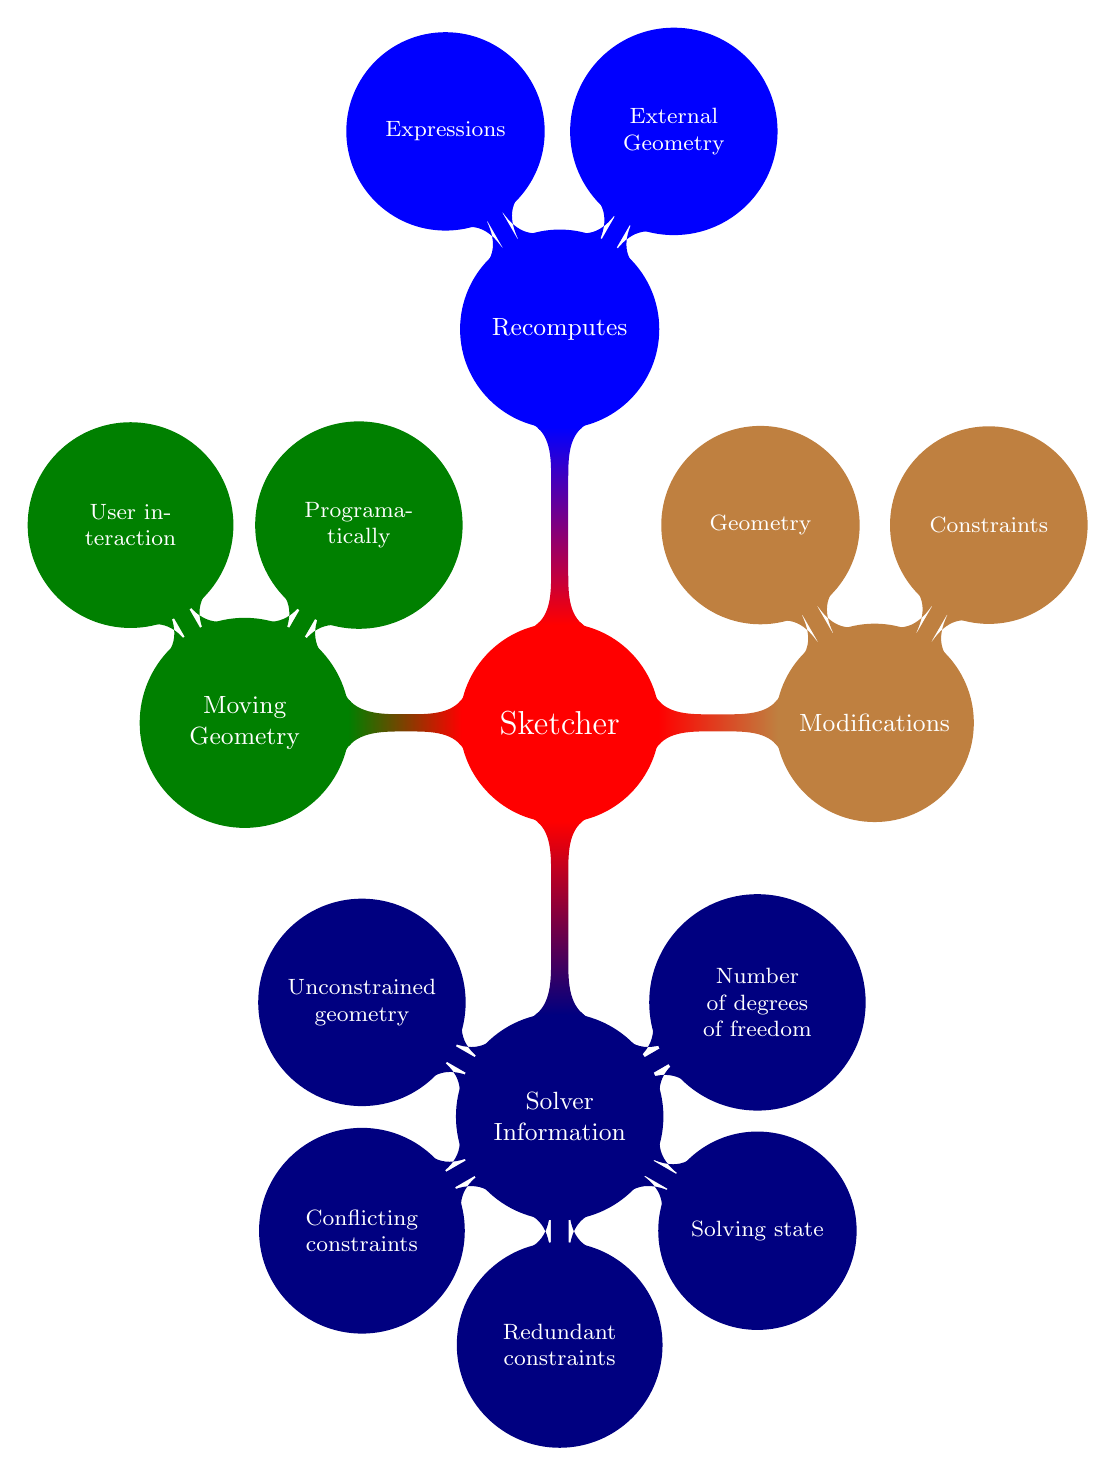
\begin{tikzpicture}
    \path[mindmap,concept color=red, text=white,
        level 1 concept/.append style = {sibling angle=90},
         every node/.append style={concept, text width=2cm, minimum size=0cm, inner sep=2mm}]
    node[concept] {Sketcher}
    [clockwise from=-90]
    child[concept color=blue!50!black] {
      node[concept] {Solver Information}
      [clockwise from=30]
      child { node[concept] {Number of degrees of freedom} }
      child { node[concept] {Solving state} }
      child { node[concept] {Redundant constraints} }
      child { node[concept] {Conflicting constraints} }
      child { node[concept] {Unconstrained geometry} }
    }
    child[concept color=green!50!black, xshift=1cm] {
      node[concept] {Moving Geometry}
      [clockwise from=120]
      child { node[concept] {User interaction} }
      child { node[concept] {Programa\-tically} }
    }
    child[concept color=blue] {
      node[concept] {Recomputes}
      [clockwise from=120]
      child { node[concept] {Expressions} }
      child { node[concept] {External Geometry} }
    }
    child[concept color=brown, xshift=-1cm] {
      node[concept] {Modifications}
      [clockwise from=120]
      child { node[concept] {Geometry} }
      child { node[concept] {Constraints} }
    };
    \end{tikzpicture}
    \end{figure}


    \section{Modifications of the Sketch}
    \label{sec:modificationsofthesketch}

    It is the most important functionality of the Sketcher, its ability to \emph{adapt} the geometry to fulfill some Sketcher constraints set by the user. One could think of how one operates while being in edit mode in the sketcher.

    In fact, there are two possibilities for solving modifications introduced while the sketcher is in edit mode: a) solving and b) recomputing. Thinking on the user interface, this is regulated by the \emph{Auto-Update} checkbox in the \emph{solver messages} task panel. When it is checked, a recompute is triggered, otherwise a solve.

    The main difference is that the recompute will propagate all the changes to the sketch to any object outside the sketcher that depends on it, while the solve will not. As a result, a solve will not change the geometry of the sketcher as seen from outside edit mode. Of course, a recompute comprises a solve, but what is relevant here is that they are separate functions.

    The c++ function implementing the \emph{solve} functionality is:

    \begin{codequote}
    int solve(bool updateGeoAfterSolving=true);
    \end{codequote}


    A call to this function involves:
    \begin{enumerate}[(i)]
     \item Resets any ongoing dragging or programatical geometry movement procedure.
        \begin{codequote}
        solvedSketch.resetInitMove();
        \end{codequote}
     \item Transfer the current values of Geometry, Constraints and ExternalGeometry to the solver interface and requests a \emph{diagnosis} of the equation system. This evaluation returns among others, the Degree of Freedom of the system and whether conflicting or redundant constraints are present. If there are redundant or conflicting constraints, or otherwise the system is overconstrained, the solving process is stopped.
        \begin{codequote}
        lastDoF = solvedSketch.setUpSketch(\\
        \-\hspace{2.5cm}getCompleteGeometry(),\\
        \-\hspace{2.5cm}Constraints.getValues(),\\
        \-\hspace{2.5cm}getExternalGeometryCount());\\

        lastHasConflict=solvedSketch.hasConflicts();\\
        lastHasRedundancies=solvedSketch.hasRedundancies();\\
        lastConflicting=solvedSketch.getConflicting();\\
        lastRedundant=solvedSketch.getRedundant();
        \end{codequote}
     \item The equations system is solved and the status retrieved. However, if the solver failed, the process continues.
       \begin{codequote}
        lastSolverStatus=solvedSketch.solve();
        \end{codequote}
     \item If the solver did not fail \underline{and} the parameter \emph{updateGeoAfterSolving} is set, the geometry of the sketch is updated based on the result of the solver.
    \end{enumerate}

    The recompute is treated in the following section together with the other cases that trigger a recompute.


    \section{Recomputes}

    When a property of an object changes, the object might have been changed and appropriate action has to be taken. The mechanism used in FreeCAD is called \emph{recompute} and the function that is executed upon recompute is:

    \begin{codequote}
    App::DocumentObjectExecReturn *execute(void);
    \end{codequote}

    A call to this function involves:
    \begin{enumerate}[(i)]
     \item Any external geometry might have changed, so the edit mode representation is updated. If such update would fail any constraint to external geometry will be removed.
        \begin{codequote}
        rebuildExternalGeometry();
        \end{codequote}
    \item A solve with \emph{updateGeoAfterSolving} set is executed. Any error originated, let it be redundant or conflicting constraints or otherwise overconstrained, or actual solver failure is notified to the user.
        \begin{codequote}
        int err = this-\textgreater{}solve(true);
        \end{codequote}
    \item In case of no errors, the bi-dimensional shape of the sketch is updated with the result obtained by the solver.
        \begin{codequote}
        Shape.setValue(solvedSketch.toShape());
        \end{codequote}
    \end{enumerate}

    The sketcher itself may trigger recomputes during edit mode in \emph{Auto-Update} mode, as described in section~\ref{sec:modificationsofthesketch}. This directly propagates all the changes in the sketch to other objects depending on it.

    Similarly, if a sketch depends on expressions or on external geometry and they change, a recompute of the sketch is generated.

    \section{Moving sketch geometry}
    \label{sec:sketcher:movingsketchgeometry}
    Sometimes it is necessary to move sketch geometry even though the solver does not require such moves in order to fulfil the constraints. This moving functionality may be the result of \emph{user interation}. One example is the operation of dragging geometry. Moving functionality is also used when the need arises to \emph{programatically} move a given geometry or one of its defined vertices. One example relates to the creation of a fillet in the sketcher. When creating a fillet it is necessary to programatically move the endpoints of the preexisting geometry to which the fillet is to be applied, to the points of start and end of the arc created to define the fillet. This must be done before any solving is performed, otherwise the solver will move both the arc and the geometry freely, resulting in unwanted behaviour.

    While the two previous functionalities directly or indirectly rely on the solving functionality of the sketcher seen before:

    \begin{codequote}
    int solve(bool updateGeoAfterSolving=true);
    \end{codequote}

    programatic moves of vertices is achieved using the \SketchObject{} function:

    \begin{codequote}
    int movePoint(int GeoId, PointPos PosId, \\
    \-\hspace{2.7cm}const Base::Vector3d\& toPoint, \\
    \-\hspace{2.7cm}bool relative=false, \\
    \-\hspace{2.7cm}bool updateGeoBeforeMoving=false);
    \end{codequote}

    A call of this function:

    \begin{enumerate}[(i)]
     \item If an update of the geometry is necessary before moving according to parameter \emph{updateGeoBeforeMoving}, solver geometry is updated. Otherwise, the geometry available at solver level is used for the moving operation.
     \item If the last execution of the solver returned an overconstrained sketch or one having conflicting constraints the moving of geometry is aborted.
     \item The solver interface point moving functionality is called. This functionality internal performs a special kind of solving, which returns a solving status.
        \begin{codequote}
        lastSolverStatus = solvedSketch.movePoint(GeoId, \\
        \-\hspace{4.5cm}PosId, toPoint, relative);
        \end{codequote}
    \item If this special solve succeeded, the geometry of the sketcher is updated based on the solution found.
     \item The solver interface moving functionality is reset as the moving operation has finished.
        \begin{codequote}
        solvedSketch.resetInitMove();
        \end{codequote}
    \end{enumerate}

    In the case of user interation, it uses a similar interface as even if it responds to user interaction, as in the end it is nothing else than a programatic move according to the input of the user. However, there are two main meaningful differences: a) it is interfaced directly from the ViewProvider, b) it uses an additional method of the \emph{solver interface}.

    The first difference is an obvious consequence of user interaction. The second one is a consequence of an ongoing move operation that requires intermediate updates. In the particular case of the drag and drop, in order to redraw during the dragging process and give the impression of interaction.

    An example of such dynamic operation can be found in \emph{ViewProviderSketch.h}:

    \begin{codequote}
    bool ViewProviderSketch::mouseMove(\\
    \-\hspace{4cm}const SbVec2s \&cursorPos,\\
    \-\hspace{4cm}Gui::View3DInventorViewer *viewer)
    \end{codequote}

    It is not worth to go into this function in detail, but it is important to identify that such operation starts with a call to the following function of the solver interface:

    \begin{codequote}
    getSketchObject()-\textgreater{}getSolvedSketch().initMove(GeoId, \\
    \-\hspace{4cm}PosId, false);
    \end{codequote}

    Subsequent calls are directly to the solver interface:

    \begin{codequote}
    getSketchObject()-\textgreater{}getSolvedSketch().movePoint(GeoId, \\
    \-\hspace{4cm}PosId, vec, false)
    \end{codequote}

    However, when the drag and drop operation ends, the final movement is effected via \emph{SketchObject} in order to update the Sketcher geometry with the solver geometry.

    \section{Sketcher relevant solver information}

    There are two types of information returned by the solver: a) general information and b) specific information. The first type is obtained every time the sketcher interface is triggered to set up a sketch or solve it. The second type is obtained only on demand after a full solving operation has finished.

    As it has been presented already in section~\ref{sec:modificationsofthesketch}, the solver must be first given the geometry it has to solve, which is performed using the \emph{setUpSketch} function of the solver interface. This function performs an initial evaluation or diagnosis of the equation system. Important information is obtained from this initial evaluation: a) the number of degrees of freedom of the system, b) whether there are redundant constraint and which ones they are, c) whether there are conflicting constraints and which ones they are.

    This information enables the Sketcher to know if it is worth trying to actually solve the system or not. However it also informs the user about the number of degrees present and which problems regarding constraints must be tackled in order to achieve a valid geometric solution.

    \begin{codequote}
        lastDoF = solvedSketch.setUpSketch(\\
        \-\hspace{2.5cm}getCompleteGeometry(),\\
        \-\hspace{2.5cm}Constraints.getValues(),\\
        \-\hspace{2.5cm}getExternalGeometryCount());\\

        lastHasConflict=solvedSketch.hasConflicts();\\
        lastHasRedundancies=solvedSketch.hasRedundancies();\\
        lastConflicting=solvedSketch.getConflicting();\\
        lastRedundant=solvedSketch.getRedundant();
    \end{codequote}

    If the diagnosis shows no problem, then the actual solving is performed and additional information is obtained:

    \begin{codequote}
        lastSolverStatus = solvedSketch.solve();
    \end{codequote}

    This status information is defined in \emph{GCS.h} and may take several values:

    \begin{itemize}
     \item \textbf{GCS::Success}: Solution zeroes the error function
     \item \textbf{GCS::Converged}: Solution minimizes the error function, but does not zero it.
     \item \textbf{GCS::Failed}: The solver failed to find a solution.
     \item \textbf{GCS::SuccessfulSolutionInvalid}: The solver found a solution, but this solution is not accepted by OpenCASCADE.
    \end{itemize}

    In practice this information is currently used only in binary form at Sketcher level, either \emph{GCS::Success} or \emph{GCS::Failed}. This information is fed back to the user in the \emph{solver messages} task panel.

    Regarding the specific information, currently the solver is capable of identifying geometry having parameters that are dependent within the definition of sections~\ref{sec:solvergeometry} and ~\ref{sec:solverconstraints}. However, this cannot be achieved with the faster algorithm that the solver uses by default for $QR$ decomposition of sparse matrices, \emph{SparseQR}. Therefore in order to achieve it a specific solve is requested with a full pivoting dense $QR$ decomposition. Asuming that \emph{Obj} below is an instance of \SketchObject{}, this specific solve may be requested by manually setting the $QR$ algorithm:

    \begin{codequote}
        Obj-\textgreater{}getSolvedSketch()\\
        \-\hspace{1cm}.setQRAlgorithm(GCS::EigenDenseQR);\\
        Obj-\textgreater{}solve(false);\\
        Obj-\textgreater{}getSolvedSketch()\\
        \-\hspace{1cm}.setQRAlgorithm(GCS::EigenSparseQR);
    \end{codequote}

    After that solve, the solver interface may be queried for a given geometry index, \emph{geoId} and a given Sketcher::PointPos, \emph{pos}, as follows:

    \begin{codequote}
        Obj-\textgreater{}getSolvedSketch()\\
        \-\hspace{1cm}.hasDependentParameters(geoId, pos);
    \end{codequote}

    A complete example of how to obtain this information is available in \emph{CommandSketcherTools.cpp}:

    \begin{codequote}
    void CmdSketcherSelectElementsWithDoFs::activated(int)
    \end{codequote}

    Alternatively, \SketchObject{} also has a function that returns a vector of geo index and PointPos pairs containing all the dependent parameters. This is also accessible from Python.

    \begin{codequote}
    void\\ SketchObject::getGeometryWithDependentParameters\\
    \-\hspace{0.75cm}(std::vector\textless{}std::pair\textless{}int,PointPos\textgreater{}\textgreater{}\& geometrymap)
    \end{codequote}

    \chapter{Solver interface}

    \section{Introduction}

    The most important function of the solver interface is that of interfacing between the sketcher (\SketchObject) and the solver (\emph{PlaneGCS}). This mainly involves translating the geometry and constraint information from its Sketcher form to a form usable by the solver before solving it and conveying the result embedded in the solver geometry back to the Sketcher. In order to effectively achieve this function, the solver interface must keep track of sketcher and solver, for which it maintains a plurality of \emph{data structures}.

    As it has already been introduced in chapter~\ref{chap:sketcherfunctions}, the solver provides interfaces to enable: a) solving, b) moving geometry and c) retrieving solver information.

    \section{Data structures}

    \subsection{Geometry}

    The geometry at Solver interface level is structured into a vector of a solver interface defined type, \emph{GeoDef} and a plurality of geometry type specific vectors containing the solver representation of each geometry:

    \begin{codequote}
    std::vector\textless{}GeoDef\textgreater{} Geoms;\\
    \\
    std::vector\textless{}GCS::Point\textgreater{}  Points;\\
    std::vector\textless{}GCS::Line\textgreater{}   Lines;\\
    std::vector\textless{}GCS::Arc\textgreater{}    Arcs;\\
    std::vector\textless{}GCS::Circle\textgreater{} Circles;\\
    std::vector\textless{}GCS::Ellipse\textgreater{} Ellipses;\\
    std::vector\textless{}GCS::ArcOfEllipse\textgreater{} ArcsOfEllipse;\\
    std::vector\textless{}GCS::ArcOfHyperbola\textgreater{} ArcsOfHyperbola;\\
    std::vector\textless{}GCS::ArcOfParabola\textgreater{} ArcsOfParabola;\\
    std::vector\textless{}GCS::BSpline\textgreater{} BSplines;
    \end{codequote}

    The solver interface defined type is a struct including a pointer to a copy of the Sketcher geometry, a solver interface defined geometry type, a flag to indicate whether the geometry is external or not, an index that corresponds to the position of this geometry within the geometry type specific vectors containing the solver representation, and an index for each of the three possible addressable vertices of a shape in the vector containing the solver representation of points.

    \begin{codequote}
    Part::Geometry  * geo;\\
    GeoType           type;\\
    bool              external;\\
    int               index;\\
    int               startPointId;\\
    int               midPointId;\\
    int               endPointId;
    \end{codequote}

    With this information the Sketcher keeps track of the geometry and enables the bidirectional synchronisation of geometry information.

    \subsection{Constraints}

    The constraints at Solver interface level are structured into a vector of a solver interface defined type, \emph{ConstrDef}.

    \begin{codequote}
    std::vector\textless{}ConstrDef\textgreater{} Constrs;
    \end{codequote}

    The solver interface defined type including a pointer the sketcher constraint, a flag indicating whether the constraint is driving or reference, a first pointer to double pointing to the memory address of a datum value of the constraint provided it has one, and a second pointer to double pointing to the memory address of a second datum value provided it has one. The latter is only used in the case of a Snell's law constraint.

    \begin{codequote}
    Constraint *    constr;\\
    bool            driving;\\
    double *        value;\\
    double *        secondvalue;
    \end{codequote}

    \subsection{Parameters}

    As it was introduced in section~\ref{sec:architecture:solver:parameters}, the solver works based on parameters. As the solver geometry is created at the solver interface, another important function of the sketcher interface is allocating memory for these parameters and keeping track of them.

    There is a first vector of pointers to double that contains all the parameters of the system that are not fixed (e.g. the parameters of external geometry), a second vector contains only those which are driven (i.e. the datums of reference constraints), a third one contains only fixed parameters (e.g. the parameters of external geometry), a fourth one contains those parameters that, after a diagnosis using the full pivoting dense QR decomposition, have been detected as being dependent parameters. Then there are two additional arrays of doubles, \underline{not} pointers to doubles, which store parameters used for programatically moving geometry.

    \begin{codequote}
    std::vector\textless{}double *\textgreater{} Parameters;\\
    std::vector\textless{}double *\textgreater{} DrivenParameters;\\
    std::vector\textless{}double *\textgreater{} FixParameters;\\
    std::vector\textless{}double *\textgreater{} pconstraintplistOut;\\
    std::vector\textless{}double\textgreater{} MoveParameters, InitParameters;
    \end{codequote}

    \section{Transfer from the sketcher to the solver}
    \label{sec:solverinterface:transferfromsketchertosolver}
     \begin{figure}
    \caption{Flow chart of setting up sketch}
    \begin{tikzpicture}[node distance=2cm]
        \node (start) [startstop] {Start};
        \node (in1) [io, below of=start] {Sketcher geometry and constraints};
        \node (pro1) [process, below of=in1, text width=8cm] {Get blocked geometry and unenforceable constraints};
        \node (pro2) [process, below of=pro1, text width=8cm] {Add geometry};
        \node (pro3) [process, below of=pro2, text width=8cm] {Add constraints};
        \node (pro4) [process, below of=pro3, text width=8cm] {Init solver and diagnose equation system};
        \node (out1) [io, below of=pro4, text width=8cm] {Retrieve redundant or conflicting constraint information and dependent parameter list};
        \node (pro5) [process, below of=out1, , text width=8cm] {Calculate geometries with dependent parameters};
        \node (stop) [startstop, below of=pro5] {Stop};
        \draw [arrow] (start) -- (in1);
        \draw [arrow] (in1) -- (pro1);
        \draw [arrow] (pro1) -- (pro2);
        \draw [arrow] (pro2) -- (pro3);
        \draw [arrow] (pro3) -- (pro4);
        \draw [arrow] (pro4) -- (out1);
        \draw [arrow] (out1) -- (pro5);
        \draw [arrow] (pro5) -- (stop);

        \begin{pgfonlayer}{background}
            \node[inner sep=10pt, surround] (background) [fit = (start) (in1) (stop) (pro2) (pro5)] {};
            % label
            \node[above left] at (background.south east) {setUpSketch()};
        \end{pgfonlayer}
    \end{tikzpicture}
    \end{figure}

    As presented in previous sections, the geometry of the Sketcher is transferred to the solver using the solver interface function:

    \begin{codequote}
        int setUpSketch(\\
        \-\hspace{0.75cm}const std::vector\textless{}Part::Geometry *\textgreater{} \&GeoList,\\
        \-\hspace{0.75cm}const std::vector\textless{}Constraint *\textgreater{} \&ConstraintList,\\
        \-\hspace{0.75cm}int extGeoCount=0);
    \end{codequote}

    The sketcher geometry is \emph{complete} geometry. This means that it includes both internal geometry and external geometry in the same vector. The internal geometry is pushed into the vector first and then the external geometry. The last parameter indicates how many external geometries are present in the vector. This allows to calculate the boundary between internal and external geometry.

    As this is the point at which geometry and constraints are added to the solver, it is also the point in which it may be decided which geometries and constraints to send to the solver. In other words, if for some reason a geometry or a constraint shall not take part in the solving procedure or shall take part but in a special way, it needs to be processed accordingly at this point. One such example is the implementation of the \emph{Block} constraint. Which sets the parameters of the blocked geometry as if they were external geometry, i.e. fixed, and excludes some other constraints as a result.

    The function to add geometry iterates the vector of geometry taking into account any blocked geometry, checks for the Sketcher type and executes a type specific addition function. A simple example illustrating this process corresponds to function:

    \begin{codequote}
    int Sketch::addLineSegment(\\
    \-\hspace{0.75cm}const Part::GeomLineSegment \&lineSegment, bool fixed)
    \end{codequote}


    The following is an example of such a specific function for a line segment. First depending on whether the geometry is external or internal, the right vector of parameter is selected. Second, a copy of the geometry is created. A
    solver interface defined type, \emph{GeoDef}, object is created and the pointer and type data assigned. Corresponding solver geometry types are created of the Points and the Line, and memory is allocated in the relevant parameters vector for the coordinates of the start and endpoints. Points are added to the points vector and the line to the lines vector. The indices of the start and endpoints in the Points array are added to the \emph{GeoDef} object, which is added to the sketcher interface vector containing all the geometries.

    \begin{codequote}
    std::vector\textless{}double *\textgreater{}\&params = \\
    \-\hspace{0.75cm}fixed ? FixParameters : Parameters;\\

    GeomLineSegment *lineSeg = \\
    \-\hspace{0.75cm}static\_cast\textless{}GeomLineSegment*\textgreater{}(lineSegment.clone());\\

    GeoDef def;\\
    def.geo  = lineSeg;\\
    def.type = Line;\\

    Base::Vector3d start = lineSeg-\textgreater{}getStartPoint();\\
    Base::Vector3d end   = lineSeg-\textgreater{}getEndPoint();\\

    GCS::Point p1, p2;\\

    params.push\_back(new double(start.x));\\
    params.push\_back(new double(start.y));\\
    p1.x = params[params.size()-2];\\
    p1.y = params[params.size()-1];\\

    params.push\_back(new double(end.x));\\
    params.push\_back(new double(end.y));\\
    p2.x = params[params.size()-2];\\
    p2.y = params[params.size()-1];\\

    def.startPointId = Points.size();\\
    def.endPointId = Points.size()+1;\\
    Points.push\_back(p1);\\
    Points.push\_back(p2);\\

    GCS::Line l;\\
    l.p1 = p1;\\
    l.p2 = p2;\\
    def.index = Lines.size();\\
    Lines.push\_back(l);\\

    Geoms.push\_back(def);\\

    return Geoms.size()-1;
    \end{codequote}

    The function to add constraints iterates the vector of constraints taking into account any unenforceable constraint. For each sketcher constraint it creates a
    solver interface defined type, \emph{ConstrDef}, object, assignes the constraint pointer and sets the driving flag accordingly. Then, the constraint type is checked. If the constraint contains datums, memory is allocated for a parameter and the value of the constraint is assigned, the parameter is assigned to the \emph{FixParameters} vector if the constraint is driving and to the \emph{Parameters} \underline{and} \emph{DrivenParameters} vectors if it is reference. This allows to enforce the constraint value in case it is driving and to let it be modified by the solver if it is reference. Datum or not, a constraint specific function is called to create the one or more corresponding solver constraints. An example of such a function is:

    \begin{codequote}
    int Sketch::addDistanceXConstraint(int geoId, \\
    \-\hspace{5.5cm}double * value, bool driving)
    \end{codequote}

    In this specific case, this constraint the horizontal distance constraint is implemented via a solver difference constraint. First it is checked that the geo index of the constraint is valid and corresponds to the right geometry type. The line is retrieved from the Lines vector using the index stored in the \emph{GeoDef} vector. A tag is created. The tag stored in the solver constraint. In a case that several solver constraints are necessary to implement the Sketcher constraint, all the solver constraints carry the same tag. This allows to map the findings of the solver for its constraints to the sketcher constraints.

    \begin{codequote}
    geoId = checkGeoId(geoId);\\

    if (Geoms[geoId].type != Line)\\
    \-\hspace{0.75cm}return -1;

    GCS::Line \&l = Lines[Geoms[geoId].index];\\

    int tag = ++ConstraintsCounter;\\
    GCSsys.addConstraintDifference(l.p1.x, l.p2.x, value, tag, driving);\\
    return ConstraintsCounter;
    \end{codequote}

    Once geometry and constraints are added to the solver, the solver interface performs an initilisation and diagnosis:

    \begin{codequote}
    GCSsys.clearByTag(-1);\\
    GCSsys.declareUnknowns(Parameters);\\
    GCSsys.declareDrivenParams(DrivenParameters);\\
    GCSsys.initSolution(defaultSolverRedundant);
    \end{codequote}

    The actual functionality provided by these solver commands will be explained in the chapter dedicated to the PlaneGCS.

    \section{Solve}
    \label{sec:Solver:solve}
    The solve function of the solver interface is executed directly from the sketcher. However it is also executed by the solver interface functions implementing the programatic movement of geometry. The function is defined in \emph{sketch.cpp}:

    \begin{codequote}
        int Sketch::solve(void)
    \end{codequote}

    The solver includes a plurality of algorithms: a) DogLeg, b) BFGS, c) Levenberg-Marquardt and d) SQP.

    From that plurality of algorithms the preferred one is executed. If it succeedes, the geometry of the sketch is updated. If not the remaining algorithms are fired one after the other until one succeedes or none does.

    \section{Transfer from the solver to the sketcher}

    Upon successful solve the geometry of the solver, the solution is applied and the geometry of the Sketcher is updated with the solution. If the update is sucessful the values of the non driving constraints need to be updated to the values found by the solver. The solution may be invalid because OpenCASCADE may not accept it. In such a case the solve and geometry are reverted.

    \begin{codequote}
    if (ret == GCS::Success) \{\\
    \-\hspace{0.5cm}GCSsys.applySolution();\\
    \-\hspace{0.5cm}    valid\_solution = updateGeometry();\\
    \-\hspace{0.5cm}   if (!valid\_solution) \{\\
    \-\hspace{1cm}        GCSsys.undoSolution();\\
    \-\hspace{1cm}        updateGeometry();\\
    \-\hspace{0.5cm}    \}\\
    \-\hspace{0.5cm}    else \{\\
    \-\hspace{1cm}        updateNonDrivingConstraints();\\
    \-\hspace{0.5cm}    \}\\
    \}
    \end{codequote}

    The update of the geometry is done by iterating the \emph{GeoDef} vector of the solver interface and using the indices to retrieve the parameters and assign them to the \underline{copy} of the Sketcher geometry in the \emph{GeoDef} structure. The geometry assignment is performed at \SketchObject{} level, using the function \emph{extractGeometry} to obtain the copy of the Sketcher geometry. The reason for this copy and assignment is twofold: a) so that the integrity of the sketcher geometry is independent of the potential solver inability to reach a solution, and b) because the Property in \SketchObject{} must be set so that the change triggers and the property history used in the undo function are properly maintained.

    \section{Programatic Movement of geometry}

    As it has been explained in section ~\ref{sec:sketcher:movingsketchgeometry}, the functions of the \emph{solver interface} dealing with programatic movement of geometry are:

    \begin{codequote}
    int Sketch::initMove(int geoId, PointPos pos, bool fine)\\
    void Sketch::resetInitMove()\\
    int Sketch::movePoint(int geoId, PointPos pos, \\
    \-\hspace{4.1cm}Base::Vector3d toPoint, bool relative)
    \end{codequote}

    The \emph{initMove} function identifies the part of the geometry to move via the geo index \emph{geoId} and the PointPos enum. The function creates new temporary\emph{solver} constraints which are given priority when finding a solution. These constraints serve the purpose of forcing a vertex or point within an edge to follow the position or vector that will be given via the \emph{movePoint}.

    A simple example to illustrate what the \emph{initMove} function does follows.

    \begin{codequote}
    if (Geoms[geoId].type == Point) \{\\
    \-\hspace{0.5cm}if (pos == start) \{\\
    \-\hspace{1cm}GCS::Point \&point = Points[Geoms[geoId].startPointId];\\
    \-\hspace{1cm}GCS::Point p0;\\
    \-\hspace{1cm}MoveParameters.resize(2); \\
    \-\hspace{1cm}p0.x = \&MoveParameters[0]; \\
    \-\hspace{1cm}p0.y = \&MoveParameters[1]; \\
    \-\hspace{1cm}*p0.x = *point.x; \\
    \-\hspace{1cm}*p0.y = *point.y; \\
    \-\hspace{1cm}GCSsys.addConstraintP2PCoincident(p0,point,-1); \\
    \-\hspace{0.5cm}\} \\
    \}
    \end{codequote}

    A point geometry may only have a part, the PointPos Sketcher::start. The point with its \emph{parameters} is retrieved from the \emph{solver} geometry. A new point, $p0$ is created and the parameters mad to point to the \emph{MoveParameters} vector. The values of these parameters are initialised to the same value as the point to move. Then a new \emph{solver} constraint is created to indicate the \emph{solver} that these two points should be at the same position. It is noted that the constraint is added with a negative tag value of $-1$. This is to indicate that this constraint takes priority over any other constraint. As it will be explained, the solver uses a special \emph{algorithm} to solve systems having priority constraints.

    The \emph{initMove} function ends with the statements:

    \begin{codequote}
    InitParameters = MoveParameters;\\
    GCSsys.initSolution();\\
    isInitMove = true;\\
    \end{codequote}

    The relevance of them will be more apparent when presenting the \emph{solver} \emph{initSolution} function. At this point it suffices to note that it initilises the equation system so as to enable the \emph{solver} algorithms to act on them.

    The actual movement of geometry is effected by the \emph{movePoint} function. Two cases are separated here, a single programatic movement of geometry and an interactive one. For a single programatic movement, there is no need to call the \emph{initMove} function above, because \emph{movePoint} checks whether the point is initialised. If it is not, it calls the \emph{initMove} function to initilise it.

    However, in the case of interactive movement, it is not desirable to initilise the solution on every movement call as it leads to unwanted results, e.g. lagging. In this case, a single solution initialisation is updated every time the movement distance from the initial point overpasses 20 times the distance initial movement, i.e. the distance indicated by the first call to the \emph{movePoint}. This mechanism prevents jumping during dragging operations.

    There are two types of movement: a) the \emph{relative} movement, in which the parameter \emph{toPoint} indicates the vector of movement from the original position, which is mostly using for \emph{interactive} movements, like dragging, b) the \emph{absolute} movement, in which the parameter \emph{toPoint} provides the position to which the initial point shall be moved.

    The internal workings are illustrated in the following example:

    \begin{codequote}
    if (relative) \{\\
    \-\hspace{0.25cm}for (int i=0; i \textless{} int(MoveParameters.size()-1); i+=2) \{\\
    \-\hspace{0.5cm}MoveParameters[i] = InitParameters[i] + toPoint.x;\\
     \-\hspace{0.5cm}MoveParameters[i+1] = InitParameters[i+1] + toPoint.y;\\
    \-\hspace{0.25cm}\}\\
    \} else if (Geoms[geoId].type == Point) \{\\
    \-\hspace{0.25cm}if (pos == start) \{\\
    \-\hspace{0.5cm}MoveParameters[0] = toPoint.x;\\
    \-\hspace{0.5cm}MoveParameters[1] = toPoint.y;\\
    \-\hspace{0.25cm}\}\\
    \}
    \end{codequote}

    The \emph{MoveParameters} vector is updated with the new position to which the point should move, in either a \emph{relative} or \emph{absolute} way.

    Expectedly, the function ends with a \emph{solve} in order to enforce the constraint created to the new position.

    It is not possible for the \emph{solver interface} to know when an interactive moving operation is finished. For this reason, the function \emph{resetInitMove} is called at \emph{Sketcher} level when operation is over.

    \section{Retrieving solver information}

    Most of the \emph{solver information} is obtained directly from the solver itself and the solver interface acts merely as buffer. This is the case of \emph{redundant} constraints, \emph{conflicting} constraints, \emph{degrees of freedom}. The buffer is relevant in that one can operate several \emph{solver} level solvings and only updating this information when it is relevant for state of the sketch. For example, if constraints are added artificially for certain operations that solver information would be worthless for the user.

    Most of the diagnosis information is obtained from the solver diagnosis triggered in function \emph{setUpSketch}. This is the case of \emph{redundant} constraints, \emph{conflicting} constraints, \emph{degrees of freedom} and \emph{dependent parameters}.

    \begin{codequote}
        int setUpSketch(\\
        \-\hspace{0.75cm}const std::vector\textless{}Part::Geometry *\textgreater{} \&GeoList,\\
        \-\hspace{0.75cm}const std::vector\textless{}Constraint *\textgreater{} \&ConstraintList,\\
        \-\hspace{0.75cm}int extGeoCount=0);
    \end{codequote}


    Regarding the geometry having parameters that are dependent within the definition of sections~\ref{sec:solvergeometry} and ~\ref{sec:solverconstraints}, the solver interface does perform a processing, in order to convert the pure \emph{parameter} information available at the \emph{solver} into \emph{sketcher} geometry information.

    \begin{codequote}
        bool hasDependentParameters(int geoId, PointPos pos) const
        void calculateDependentParametersElements(void)
    \end{codequote}

     The function \emph{calculateDependentParametersElements} iterates the geometry structures at \emph{solver interface} level, \emph{std::vector\textless{}GeoDef\textgreater{} Geoms}. For each geometry it looks if the \emph{parameters} identified by the solver as dependent belong to the geometry, and sets the flag \emph{hasDependentParameters} accordingly. This maps the individual parameters to the geometry elements at \emph{solver interface} level that contain them. In addition to that, it further identifies the vertices of each geometry addressable via \emph{PointPos}, and sets the vertices as dependent according to the \emph{parameters} of the vertices. This enables to have information on geometric elements and the vertices separatedly.

     The function \emph{hasDependentParameters} relies on this calculation to map these \emph{solver interface} level geometry to actual \emph{Sketcher} geometry. The function returns \emph{true} or \emph{false} whether the \emph{Sketcher} geometry identified by the \emph{GeoId} index and the \emph{PointPos}.


    \chapter{PlaneGCS}

    \section{Introduction}

    The sketcher interfaces with the solver interface, which in turn interfaces with the solver. The solver holds all solver constraints and information about partitioning them into subsystems and other solution strategies, and is responsible for applying those strategies so as to obtain a valid solution.


    \section{Data structures}

    \subsection{Introduction}

    From a data member point of view, \SketchObject, defined in \emph{SketchObject.h}, has a data member which is of solver interface type, i.e. \emph{sketch}, as defined in \emph{sketch.h}. In turn the solver interface type, \emph{sketch}, has a data member of solver type \emph{GCS::System} as defined in \emph{GCS.h}.

    The most important data structures of the solver are presented below.

    When dealing with constraints, the solver constraints are stored in a vector of pointers to those constraints. Upon pushing a new constraint to the constraint vector, two adjacency lists are created, so that given a pointer to the constraint the parameters can be obtained, or given a parameter, the constraints involved.

    \begin{codequote}
    std::vector\textless{}Constraint *\textgreater{} clist;\\
    std::map\textless{}Constraint *,VEC\_pD \textgreater{} c2p;\\
    std::map\textless{}double *,std::vector\textless{}Constraint *\textgreater{} \textgreater{} p2c;
    \end{codequote}

    The vector \emph{plist} points to the list of parameters of the solver. The vector \emph{pdrivenlist} points to the subset of parameters of the solver that are the datums of reference constraints. They are set from the solver interface using the function \emph{declareDrivenParams}.

    When dealing with parameters, certain operations take advantage of a map of parameters \emph{pIndex}, in which parameters act as key and the map returns the index in the parameters vector of the given parameter. This map is generated by the \emph{declareUnknowns} function.

    Before undertaking any solving operation, the solver stores the values of the parameters in a vector of doubles \emph{reference} using the function \emph{setReferences}. This allows to revert the parameters to the reference values using the function \emph{resetToReference}.

    \begin{codequote}
    VEC\_pD plist;\\
    VEC\_pD pdrivenlist\\
    MAP\_pD\_I pIndex;\\
    VEC\_D reference;
    \end{codequote}

    \subsection{Constraint structure}

    Constraints are the basis of the solver. In section~\ref{sec:solverconstraints} the core solving functionality of solver constraints was introduced. However, several aspects regarding the general structure of the constraints will be presented here.

    All solver constraints derive from the Constraint class, which is defined as follows:

    \begin{codequote}
    class Constraint\\
    \{\\
    protected:\\
    \-\hspace{0.5cm}VEC\_pD origpvec; \\
    \-\hspace{0.5cm}VEC\_pD pvec; \\
    \-\hspace{0.5cm}double scale; \\
    \-\hspace{0.5cm}int tag; \\
    \-\hspace{0.5cm}bool pvecChangedFlag; \\
    \-\hspace{0.5cm}bool driving; \\
    public: \\
    \-\hspace{0.5cm}Constraint(); \\
    \-\hspace{0.5cm}virtual ~Constraint()\{\} \\

    \-\hspace{0.5cm}inline VEC\_pD params() \{ return pvec; \}\\

    \-\hspace{0.5cm}void redirectParams(MAP\_pD\_pD redirectionmap);\\
    \-\hspace{0.5cm}void revertParams();\\
    \-\hspace{0.5cm}void setTag(int tagId) \{ tag = tagId; \}\\
    \-\hspace{0.5cm}int getTag() \{ return tag; \}\\

    \-\hspace{0.5cm}void setDriving(bool isdriving) \{ driving = isdriving; \}\\
    \-\hspace{0.5cm}bool isDriving() const \{ return driving; \}\\

    \-\hspace{0.5cm}virtual ConstraintType getTypeId(); \\
    \-\hspace{0.5cm}virtual void rescale(double coef=1.); \\
    \-\hspace{0.5cm}virtual double error(); \\
    \-\hspace{0.5cm}virtual double grad(double *); \\
    \-\hspace{0.5cm}virtual double maxStep(MAP\_pD\_D \&dir, double lim=1.); \\
    \-\hspace{0.5cm}int findParamInPvec(double* param); \\
    \};
    \end{codequote}

    A constraint stores a first set of parameters of the constraint with the original values of the parameters, \emph{origpvec} and a second set of parameters with the current values, \emph{pvec}. The first set is only used as reference for reverting or redirecting the current values in the second set.

    A constraint also has a scale, used to scale the error and gradients. This scale may be modified using the \emph{rescale} method.

    The \emph{tag} is an index used to map solver constraints to sketcher level constraints. Additionally, negative values are used for priority constraints which behave specially and are not considered during the diagnosis of the equation system. Such priority constraints are used for example for programatically moving the geometry. It may be interfaced via the \emph{setTag} and \emph{getTag} functions.

    The flag \emph{pvecChangedFlag} indicates that the \emph{pvec} vector has changed and any saved geometry pointers in the class shall be reconstructed.

    The flag \emph{driving} indicates whether the constraint is driven or reference. It may be interfaced via the \emph{setDriving} and \emph{isDriving} functions.

    The function \emph{params} returns a vector to double pointers containing all the constraint parameters.

    The constraint has a function to return its type, which is one of the values of the enum \emph{GCS::ConstraintType}.

    The function \emph{findParamInPvec} unsurprisingly searches for a given parameter in the parameters of the constraint, and returns the index of the first occurrence, and -1 if not found.

    The function \emph{revertParams} resets the parameters vector to the original parameters.

    The function \emph{redirectParams} changes the parameters of the constraint with other parameters according to a map. Basically, it searches the parameters of the constraint as key in the map and if there is a coincidence the parameter is assigned associated the parameter in the map.

    A practical example of a constraint implementation reuses the basic functionality of the parent class and only defines a few parameters.

    \begin{codequote}
    class ConstraintDifference : public Constraint\\
    \{\\
    private:\\
    \-\hspace{0.5cm}inline double* param1() \{ return pvec[0]; \}\\
    \-\hspace{0.5cm}inline double* param2() \{ return pvec[1]; \}\\
    \-\hspace{0.5cm}inline double* difference() \{ return pvec[2]; \}\\
    public:\\
    \-\hspace{0.5cm}ConstraintDifference(double *p1, double *p2, double *d);\\
    \-\hspace{0.5cm}virtual ConstraintType getTypeId();\\
    \-\hspace{0.5cm}virtual void rescale(double coef=1.);\\
    \-\hspace{0.5cm}virtual double error();\\
    \-\hspace{0.5cm}virtual double grad(double *);\\
    \};
    \end{codequote}

    The constraint uses three parameters, \emph{p1}, \emph{p2} and \emph{d}. Its goal is to maintain a difference between those two parameters.

    The constructor basically assigns the parameters to the \emph{pvec} and initializes \emph{origpvec} to the same parameters. The member functions above are just named accessors to the parameters.

    Given the simplicity of the constraint, it is interesting to look into the error and gradient functions:

    \begin{codequote}
    double ConstraintDifference::error()\\
    \{\\
    \-\hspace{0.5cm}return scale * (*param2() - *param1() - *difference());\\
    \}\\

    double ConstraintDifference::grad(double *param)\\
    \{\\
    \-\hspace{0.5cm}double deriv=0.;\\
    \-\hspace{0.5cm}if (param == param1()) deriv += -1;\\
    \-\hspace{0.5cm}if (param == param2()) deriv += 1;\\
    \-\hspace{0.5cm}if (param == difference()) deriv += -1;\\
    \-\hspace{0.5cm}return scale * deriv;\\
    \}
    \end{codequote}

    \section{Transfer from the solver interface to the solver}
    \label{sec:solver:transferfromsolverinterfacetosolver}

    \subsection{Introduction}
    It was already introduced in section~\ref{sec:solverinterface:transferfromsketchertosolver} how the geometry and constraints were transferred from the sketcher to the solver interface. While the geometry was allocated into \emph{parameters} fully at solver interface level, the transfer of the constraints relied on specific functions of the solver itself.

    \subsection{Constraint creation}

    In the example presented above, the function responsible for adding a given constraint to the solver was implemented as:

    \begin{codequote}
    geoId = checkGeoId(geoId);\\

    if (Geoms[geoId].type != Line)\\
    \-\hspace{0.75cm}return -1;

    GCS::Line \&l = Lines[Geoms[geoId].index];\\

    int tag = ++ConstraintsCounter;\\
    GCSsys.addConstraintDifference(l.p1.x, l.p2.x, value, tag,\\
    \-\hspace{0.75cm}driving);\\
    return ConstraintsCounter;
    \end{codequote}

    In this example the \emph{addConstraintDifference} function is an example of function of the solver that ultimately implements the creation of a corresponding solver constraint:

    \begin{codequote}
    int System::addConstraintDifference(double *param1, \\
    \-\hspace{0.75cm}double *param2, double *difference, int tagId,\\
    \-\hspace{0.75cm}bool driving)
    \end{codequote}

    This function allocates dynamic memory for the solver constraint, and adds the parameters given in the constructor to the \emph{pvec} of the constraint. Then stores the tag and driving information therein and relies on a generic solver function \emph{addConstraint} to add the constraint to the system.

    \begin{codequote}
    Constraint *constr = new ConstraintDifference(param1,\\
    \-\hspace{0.75cm}param2, difference);\\
    constr-\textgreater(tagId);\\
    constr-\textgreater{}setDriving(driving);\\
    return addConstraint(constr);
    \end{codequote}


    \subsection{Constraint adition}

    This generic solver function resets the previous diagnose results if a new constraint is added, unless it has a \underline{negative} tag. As previously presented tags are mechanism to map solver constraints to sketcher constraints. However, in addition to that function, negative tags are used to mark solver constraints that do not relate to sketcher constraints, but that are artificially added to achieve a certain functionality. One example is the programatic geometry moving functionality. These constraints, which are only temporarely added do not affect the diagnosis information of the equation system in a way meaningful to the user or the solving process.

    The function pushes the new constraint into the vector of solver constraint, and adds the parameters involved in that constraint and the constraint to the adjancency lists of parameters and constraints.

    \begin{codequote}
    isInit = false;\\
    if (constr-\textgreater{}getTag() \textgreater= 0)\\
    \-\hspace{0.75cm}hasDiagnosis = false;\\

    clist.push\_back(constr);\\
    VEC\_pD constr\_params = constr-\textgreater{}params();\\

    for (VEC\_pD::const\_iterator param=constr\_params.begin();\\
    \-\hspace{0.5cm}param != constr\_params.end(); ++param) \{\\
    \-\hspace{0.75cm}c2p[constr].push\_back(*param);\\
    \-\hspace{0.75cm}p2c[*param].push\_back(constr);\\
    \}\\
    return clist.size()-1;
    \end{codequote}

    \section{Initialize the solution and diagnosis}
    \label{sec:solver:diagnosis}
    \begin{figure}
    \caption{Flow chart of solution initialisation}
    \begin{tikzpicture}[node distance=2cm]
        \node (start) [startstop] {Start};
        \node (in1) [io, below of=start] {solver parameters and constraints};
        \node (pro1) [process, below of=in1, text width=8cm] {Diagnosis};
        \node (pro2) [process, below of=pro1, text width=8cm] {Partitioning into decoupled components};
        \node (pro3) [process, below of=pro2, text width=8cm] {Identification of equality constraints and parameter reduction};
        \node (pro4) [process, below of=pro3, text width=8cm] {Organisation in subsystems};
        \node (out1) [io, below of=pro4, text width=8cm] {Subsystems \\(subSystems and subSystemsAux)};
        \node (stop) [startstop, below of=out1] {Stop};
        \draw [arrow] (start) -- (in1);
        \draw [arrow] (in1) -- (pro1);
        \draw [arrow] (pro1) -- (pro2);
        \draw [arrow] (pro2) -- (pro3);
        \draw [arrow] (pro3) -- (pro4);
        \draw [arrow] (pro4) -- (out1);
        \draw [arrow] (out1) -- (stop);

        \begin{pgfonlayer}{background}
            \node[inner sep=10pt, surround] (background) [fit = (start) (in1) (stop) (pro2) (pro5)] {};
            % label
            \node[above left] at (background.south east) {initSolution()};
        \end{pgfonlayer}
    \end{tikzpicture}
    \end{figure}

    Returning to the sketcher interface function \emph{setUpSketch} in section ~\ref{sec:solverinterface:transferfromsketchertosolver}, there were some lines of code after the transfer of geometry and constraints to the solver that were not explained in that section.

    \begin{codequote}
    GCSsys.clearByTag(-1);\\
    GCSsys.declareUnknowns(Parameters);\\
    GCSsys.declareDrivenParams(DrivenParameters);\\
    GCSsys.initSolution(defaultSolverRedundant);
    \end{codequote}

    The first line of code clears any constraint having a priority tag with value -1. After any eventual deletion the code cares so that the constraint to parameter adjacency lists are updated. This effectively removes from the system any constraint that might have been added to programatically move geometry.

    The \emph{declareUnknowns} function initializes the \emph{pIndex} map.

    The \emph{declareDrivenParams} function sets the subset of parameters that are datums of driven constraints.

    The \emph{initSolution} function is rather complex and performs the following operations:

    \begin{itemize}
     \item Stores the current parameters values in the vector \emph{reference}
     \item Performs a diagnosis of the whole equation system using a $QR$ decomposition, thereby identifying the degrees of freedom, redundant and conflicting constraints and optionally dependent parameters.
     \item Identifies any decoupled subsystems and partitions the original system into corresponding components
     \item Identifies the equality constraints tagged with $ids >= 0$ and prepares a corresponding system reduction
     \item Organizes the rest of constraints into two subsystems for tag $ids >=0$ and $< 0$ respectively
    \end{itemize}

    \subsection{Diagnosis}

    Diagnosing an equation system as the one of the solver is a rather complex procedure. The function that implements the diagnosis is:

    \begin{codequote}
    int System::diagnose(Algorithm alg)
    \end{codequote}

    The objective of the diagnosis is to detect redundant and conflicting constraints and calculate the degrees of freedom of the equation system. Optionally, it is possible to also identify parameters that are not fully constrained.

    \begin{figure}
    \caption{Flow chart of equation system diagnosis}
    \begin{tikzpicture}[node distance=2cm]
        \node (start) [startstop] {Start};
        \node (in1) [io, below of=start] {solver parameters and constraints};
        \node (pro1) [process, below of=in1, text width=8cm] {Construct Jacobian matrix};
        \node (pro2) [process, below of=pro1, text width=8cm] {Perform QR decomposition of the Jacobian matrix};
        \node (pro3) [process, below of=pro2, text width=8cm] {Determine dependent parameters};
        \node (pro4) [process, below of=pro3, text width=8cm] {Determine redundant/conflicting constraints};
        \node (out1) [io, below of=pro4, text width=8cm] {Rank, redundant constraints, conflicting constraints, dependent parameters};
        \node (stop) [startstop, below of=out1] {Stop};
        \draw [arrow] (start) -- (in1);
        \draw [arrow] (in1) -- (pro1);
        \draw [arrow] (pro1) -- (pro2);
        \draw [arrow] (pro2) -- (pro3);
        \draw [arrow] (pro3) -- (pro4);
        \draw [arrow] (pro4) -- (out1);
        \draw [arrow] (out1) -- (stop);

        \begin{pgfonlayer}{background}
            \node[inner sep=10pt, surround] (background) [fit = (start) (in1) (stop) (pro2) (pro5)] {};
            % label
            \node[above left] at (background.south east) {diagnose()};
        \end{pgfonlayer}
    \end{tikzpicture}
    \end{figure}


    As already anticipate in previous sections, the diagnosis of the equation system is performed using the Jacobian matrix of the system, which is nothing else than a matrix having the gradients of each constraint respect to each of the parameters. Knowing that most constraints only depent on a reduced number of parameters, it is not surprising that such a matrix is substantially sparse (it has a lot of elements that are zero). This is why it is interesting to support sparse algorithms, as they are much more efficient from a computational point of view.

    The Jacobian matrix, which is generally a non-square matrix (it has dimensions of the number of constraints times the number of parameters) is decomposed into a $QR$ form. The $QR$ decomposition is a rank-reveling decomposition, meaning that it enables to obtain the rank and thus the degrees of freedom of the equation system. In general, the $QR$ decomposition of the Jacobian matrix $J$ implies finding an orthonormal matrix $Q$ that multiplied by trapezoidal matrix $R$ gives the Jacobian matrix $J$, so $J=QR$. The trapezoidal matrix $R$ is formed by an upper triangular matrix with zeros at the bottom.

    There are different algorithms to obtain a $QR$ decomposition. Different algorithms and variants of such decompositions. Some of the feature \emph{pivoting} or \emph{full pivoting}. Some are dense algorithms, i.e. algorithms designed for dense matrices, while others are sparse algorithms designed for sparse matrices. Unsurprisingly different algorithms provide a different amount of additional information.

    In general the $QR$ decomposition involves matrix operations of transposition and permutation. This operations cause that the rows and columns of the $Q$ and $R$ matrices do not correspond to the rows and columns of the $J$, even though their product sucessfully produces $J$. Due to the type of matrix, this information is specially important to extract additional information from the trapezoidal matrix $R$, like the actual constraints that are redundant or conflicting or the parameters that are not fully constraint, i.e. the dependent parameters of the system.

    The dense algorithm for $QR$ decomposition is Eigen's \emph{FullPivHouseholderQR}. This decomposition is of the type $PJP'=QR$, where $P$ and $P'$ are permutation matrices. This algorithm enables to obtain information about the dependent parameters of the system.

    The sparse algorithm for $QR$ decomposition is Eigen's \emph{SparseQR}. This decomposition is of the type $JP'=QR$, where $P'$ is the column permutation which is the product of the fill-reducing and the rank-revealing permutations.

    One historical source of problems in the diagnosis were the reference constraints, which are referred to as driven constraints in the code. Driven constraints create by definition dependent rows, as their datum value is not enforced, while they artificially enlarge the number of parameters and constraints when compared with a case not having such constraints. These problems were addressed by removing the driven constraints from the diagnose. Therefore the diagnose does not operate directly on the parameters vector \emph{plist}, but on a reduced version \emph{pdiagnoselist}.

    Removing the reference constraints has the drawback that it makes difficult to identify the solver constraints detected as redundant or conflicting by index. In order to overcome that limitation, a map \emph{jacobianconstraintmap} is created, which assign the index within \emph{plist} to each key having the corresponding index within \emph{pdiagnoselist}.

    When redundant or conflict constraints are detected, it is relevant to know whether those redundant or conflicting solver constraints correspond to a single sketcher level constraint, or if the corresponding sketcher level constraint gave rise to a plurality of solver constraints. For this reason, the diagnose function makes use of a \emph{tagmultiplicity} map, which maps the number of solver constraints to a key that is the tag of the constraint.

    The Jacobian matrix is created by calculating for each constraint and each parameter, the gradient of the constraint with respect to the parameter:

    \begin{codequote}
    J(jacobianconstraintcount-1,j) = \\
    \-\hspace{4.5cm}(*constr)-\textgreater{}grad(pdiagnoselist[j]);
    \end{codequote}

    Once the Jacobian matrix is created, Eigen is used to calculate the $QR$ decomposition. For reason relating to the availability of permutation information in the different algorithms, a transposed Jacobian matrix is what is actually decomposed. The only effect is that the parameters appear as rows in the decompositions while the constraints appear as columns. The advantage is that column permutation information is available for all the algorithms used.

    \begin{codequote}
    qrJT.compute(\\
    \-\hspace{2cm}J.topRows(jacobianconstraintcount).transpose());\\

    paramsNum = qrJT.rows();\\
    constrNum = qrJT.cols();\\

    qrJT.setThreshold(qrpivotThreshold);\\
    rank = qrJT.rank();\\

    if (constrNum \textgreater{}= paramsNum)\\
    \-\hspace{0.5cm}R = qrJT.matrixQR().triangularView\textless{}Eigen::Upper\textgreater{}();\\
    else\\
    \-\hspace{0.5cm}R = qrJT.matrixQR().topRows(constrNum)\\
    \-\hspace{2cm}.triangularView\textless{}Eigen::Upper\textgreater{}();\\
    \end{codequote}

    From a practical point of view, it is worth mentioning that in order to determine the rank, the algorithm uses a threshold, which filters out the numbers that while being negligible are not zero. This threshold that is configurable is usually set at around $10^{-13}$. Another particularity is that the R matrix in the code is the upper triangular matrix of the trapezoidal matrix.

    When using the dense algorithm, Eigen provides the transpositions matrix of the rows. The rows correspond to the parameters, as the QR decomposition was performed on the transposed matrix. With the transposition matrix it is possible to calculate the corresponding permutation matrix of the rows, which can be used to map the parameters corresponding to the rows of the $R$ matrix to the parameters of the $J$ matrix.

    The first \emph{rank} rows of the $R$ matrix correspond to the parameters that are fully constrained and form linearly independent columns in the transposed Jacobian matrix. The remaining parameters are the ones that are not fully constrained or dependent parameters, and thus do not contribute to the rank of the system. These dependent parameters are stored in \emph{pdependentparameters}.

    Unfortunately, this parameter detection does not seem to work when using the SparseQR algorithm. It may well be that it is not possible or that simply nobody of us have come with the right solution.

    The diagnose algorithm continues with the detection of conflicting or redundant constraints. If the number of constraints exceeds the rank of the system, there are necessarily redundant or conflicting constraints.

    Just for this paragraph considering that a trapezoidal $R$ matrix, and from the point of view of algebra and taking into consideration that our $QR$ decomposition was performed on transposed Jacobian matrix having $N$ rows corresponding to the $N$ parameters of the system and $M$ columns corresponding to the $M$ constraints, the $Q$ matrix must also have $N$ rows, and the $R$ matrix must also have $M$ columns. Although it is not relevant for the discussion, it is worth noting that the number of colunms of the $Q$ matrix and the number of rows of the $R$ matrix is the same value (otherwise $Q$ could not be right multiplied by $R$) and that value depends on the rank of the system. The $R$ matrix has a first number of rows that corresponds to the upper triangular matrix and a second number of rows which are zero. The values at the diagonal of this upper triangular matrix will be refered to as \emph{pivots} in the sucessive. By definition in an upper triangular matrix all elements under the pivots, i.e. under the diagonal, are zero. However, the values above the diagonal may take any value. Looking at the first column, it has just one non-zero value, the first one. If we think about how the $Q$ matrix will be right multiplied by the $R$ matrix to produce the transposed jacobian matrix, the values of the first column of it will be determined just on the basis of this non-zero value. It is possible to perform zero reduction operations on the triangular matrix by applying transposition operations. This zero reduction will show that some independent parameters are being defined by more than one constraint, the non-zero values that appear on the upper triangular matrix $R$ after zero reduction, indicating which constraints. This means that either those constraints are conflicting or they are redundant. It is possible to use the column permutation matrix provided by Eigen, in order to map the columns of $R$ with the original constraint from which they have originated. This way it is possible to determine which \emph{solver} constraints are redundant. As more than one non-zero value may actually appear after zero reduction, several \emph{solver} constraints may be conflicting or redundant for a single degree of freedom removed. Therefore, groups of constraints are identified. In the code, this vector of groups is called:

\begin{codequote}
    std::vector\textless{} std::vector\textless{}Constraint *\textgreater{}\textgreater{}\\ \-\hspace{4cm}conflictGroups(constrNum-rank);
\end{codequote}

    The name must seem misleading given the fact that it is not known at this point whether they are redundant or conflicting. In order to detect whether the constraints are redundant or conflicting, the idea is to remove the constraints and try to solve the system, if the error of the constraints is small despite the constraints not having intervened in the solving process, the constraints were \emph{redundant}, whereas if the error is large, they were conflicting. This solution finding is known in the user interface as \emph{redundant solving}, and uses the same algorithms that a normal solving, which will be introduced later on, albeit with differences. These differences will be considered later in the document. It suffices to note that one of the parameters taken by the solving algorithms is just indicating a redundant solving.

    There is one main problem remaining before solving. The previous algorithm returns groups of constraints that are conflicting or redundant within the group. However, when two constraints are redundant, a decision must be taken as to which one of them is to be removed. Additionally, a same \emph{solver constraint} may affect several groups. In order to address this problem a heuristic algorithm is executed on these groups until enough constraints have been identified for removal. This identifies for removal the constraints according to these priority rules:

    \begin{itemize}
     \item the constraints that are more popular, i.e. that appear the most among the groups.
     \item when the popularity is the same, those having a tag with lower multiplicity, i.e. those associated with sketcher constraints that generated a lower number of solver constraints.
     \item when the popularity and the multiplicity are the same, those with a higher tag number, i.e. those introduced the latest a Sketcher level.
    \end{itemize}

    The rationale behind this heuristic algorithm is that if there are several problems, the constraint intervening the most in those problems is the culprit. If there are several such constraints intervening the same amount of times in those problems, it is preferable to get rid of \emph{solver} constraints associated with \emph{sketcher} constraints that generated a lower amount of \emph{solver} constraints. The principle is that the \emph{solver} constraint associated to the less complex \emph{sketcher} constraint should be eliminated, as a \emph{sketcher} constraint may be \underline{partly} redundant with another \emph{sketcher} constraint, i.e. it may generate a plurality of \emph{solver} constraints, where one of such \emph{solver} constraints is redundant with the \emph{solver} constraints generated from the other \emph{sketcher} constraint, while the others are not. Finally, if the popularity and the multiplicity are the same, the one introduced the latest in the sketcher is chosen. This criteria is the least relevant one, but as one should be chosen anyway, it assumes that the user will have a better change to adapting to the prospective removal of the constraint introduced most recently out of those redundant. It is noted that this paragraph refers to redundancy, but it is still not known whether the constraints are redundant or conflicting.

    In order to determine whether the constraints chosen to be removed are redundant or conflicting, an equation system is built without them and a solution is found. If such solution exists, the error of each constraint is checked, and those constraints with an error under the threshold of \emph{convergence} for redundant solving are marked as redundant \emph{solver} constraints.

    \begin{codequote}
    SubSystem *subSysTmp = new SubSystem(clistTmp, pdiagnoselist);\\
    int res = solve(subSysTmp,true,alg,true);
    \end{codequote}

    From a programming perspective it is worth mentioning that after solving the solution is applied, the error obtained and after the determination of whether the constraint is redundant or conflicting is made, the parameters are reset to reference values, so that this solving does not affect the solution that will be calculated as described in the following sections.

    \begin{codequote}
    subSysTmp-\textgreater{}applySolution();\\
    for (std::set\textless{} *\textgreater{}::const\_iterator constr=skipped.begin();\\
    \-\hspace{1.5cm}constr != skipped.end(); ++constr) \{\\
    \-\hspace{0.5cm}double err = (*constr)-\textgreater{}error();\\
    \-\hspace{0.5cm}if (err * err \textless{} convergenceRedundant)\\
    \-\hspace{1cm}redundant.insert(*constr);\\
    \}\\
    resetToReference();
    \end{codequote}

    The redundant constraint set is stored and will be used in other functions within the \emph{initSolution} process.

    However, information about the redundant and conflicting constraints is separatedly stored to be retrievable by the \emph{solver interface} and the \emph{sketcher}, in order to inform the user. This information is different from the redundant and conflicting information referred to above in that:

    \begin{itemize}
     \item Conflicting constraints with tag equal to zero are not reported.
     \item Redundant \emph{solver} constraints associated to a tag comprising other non-redundant \emph{solver} constraints are not reported, i.e. they originate from a \emph{Sketcher} constraint that is partially redundant. The rationale is that there is not point in telling the user that a constraint he cannot remove is partially redundant. There is nothing the user can do about it.
    \end{itemize}

    \subsection{Partitioning into decoupled components}

    The diagnose process determines redundant constraints, which are removed from the constraint system in order to partion the system into decoupled components. This includes the \emph{solver} constraints that originated from \emph{partially} redundant \emph{sketcher} constraints.

    The consequence is that if a \emph{sketcher} constraint is partially redundant, the redundant part is automatically removed. If a \emph{sketcher} constraint is fully redundant, it is reported. It has been asked several times why not have the solver ignore the redudant constraints altogether. The answer is that eliminating \emph{sketcher} constraints helps prevent more complex problems and helps the user have cleaner sketches.

    The decoupling into components is effected using a graph. First a vertex is added per parameter and per constraint. Then, for each constraint, the adjacent parameters are iterated and an edge is created connecting the corresponding constraint vertex with the index the index in the parameters vector of the given parameter.

    This enables to determine how many components, unconnected vertices, are present.

    \subsection{Identification of equality constraints and parameter reduction}

    Parameter reduction is effected by eliminating constraints by reduction. The eliminated constraints are stored in:

    \begin{codequote}
    std::set\textless{}Constraint *\textgreater{} reducedConstrs;
    \end{codequote}

    These parameter reductions are calculated and stored in a vector of maps called \emph{reductionmaps}, storing a reductionmap per component, i.e. decoupled subsystem.

    \begin{codequote}
    std::vector\textless{} std::map \textless{} double * , double *\textgreater{}\textgreater{} reductionmaps;
    \end{codequote}

    The reduction map is calculated by iterating the \emph{solver} constraints and for those that are equality constraints, the first parameter is kept, while the second parameter is reduced. This means that the second parameter is made to point to the first parameter. For each of the components this association of reduced parameters is stored in the map.

    The parameters and constraints after reduction are stored in \emph{clists} and \emph{plists} respectively. This includes, per component, all the constraints that are not the reduced ones.

    \subsection{Organisation in subsystems}

    This step uses the information of parameters and constraints after reduction together with the \emph{reductionmaps} in order to organise the resulting parameters and constraints into subsystems.

    As explained in previous sections, the actual subsystems to be solved are stored in vectors of \emph{GCS::SubSystem} type.

    \begin{codequote}
    std::vector\textless{}SubSystem *\textgreater{} subSystems, subSystemsAux;
    \end{codequote}

    These vectors are first cleared and any previously allocated memory released. Then the \emph{reduced} constraints per decoupled component are iterated. Two subsystems per component are created, one stored into \emph{subSystems} and the other stored into \emph{subSystemsAux}. The former containts the subsystems formed by the \emph{reduced} constraints with non-negative tags, whereas the latter contains the subsystems formed by the \emph{reduced} constraints with negative tags. As explained before the constraints with negative tag originate from programatic movements of geometry.

    \section{Solve}

    There is one \emph{general} solving function at \emph{solver} level. There are three \emph{specific} solving functions intended for special circumnstances and to be used by the \emph{general} solving function. There are four \emph{algorithms} that implement modified newton methods to perform the actual solving.

    \subsection{Parameter solve}

    The first \emph{specific} solving function takes the \emph{parameters} to solve. It initializes a solution for those parameters and solves the system using the \emph{general} solving function. Hence, the specific part is the particular initilization directly from \emph{parameters}. This function is currently \emph{not} used by FreeCAD.

    \begin{codequote}
    int System::solve(VEC\_pD \&params,\\
    \-\hspace{3cm}bool isFine,\\
    \-\hspace{3cm}Algorithm alg,\\
    \-\hspace{3cm}bool isRedundantsolving)
    \end{codequote}

    \subsection{Single subsystem solve}

    The second \emph{specific} solving function takes one subsystem with no priority constraints, i.e. without any constraint with negative tags. This function is also the function used for the \emph{redundant} solvings to determine whether a constraint is \emph{redundant} or \emph{conflicting} during the \emph{diagnose} (see section ~\ref{sec:solver:diagnosis}). The actual function is:

    \begin{codequote}
    int System::solve(SubSystem *subsys,\\
    \-\hspace{3cm}bool isFine,\\
    \-\hspace{3cm}Algorithm alg,\\
    \-\hspace{3cm}bool isRedundantsolving)
    \end{codequote}

    Solving a single subsystem is the most frequent solving operation and just relies on the actual implementation of the solving \emph{algorithms} implemented for a single subsystem solving. Currently, those algorithms are:

    \begin{itemize}
     \item \emph{Broyden-Fletcher-Goldfarb-Shanno}, BFGS in the following.
     \item \emph{Levenberg-Marquardt}, LM in the following.
     \item \emph{DogLeg}, DL in the following.
    \end{itemize}


    The functions implementing those \emph{algorithms} are:

    \begin{codequote}
    int System::solve\_BFGS(SubSystem *subsys,\\
    \-\hspace{3cm}bool /*isFine*/, \\
    \-\hspace{3cm}bool isRedundantsolving)\\
    \\
    int System::solve\_LM(SubSystem* subsys,\\
    \-\hspace{3cm}bool isRedundantsolving)\\
    \\
    int System::solve\_DL(SubSystem* subsys,\\
    \-\hspace{3cm}bool isRedundantsolving)
    \end{codequote}

    \subsection{Two subsystem solving}

    The third \emph{specific} solving function is actually the implementation of an \emph{algorithm}. This is because there is only one \emph{algorithm} for the simultaneous solving of two subsystems. The algorithm gives priority to one subsystem over the other. This is the algorithm used for \emph{programatic} moving operations like dragging. The function is:

    \begin{codequote}
    int System::solve(SubSystem *subsysA,\\
    \-\hspace{3cm}SubSystem *subsysB,\\
    \-\hspace{3cm}bool /*isFine*/,\\
    \-\hspace{3cm}bool isRedundantsolving)
    \end{codequote}


    \subsection{General solve}

    The function that is called by the \emph{solver interface} in order to effect a solve operation as seen in section ~\ref{sec:Solver:solve} is:

    \begin{codequote}
    int System::solve(bool isFine,\\
    \-\hspace{3cm}Algorithm alg,\\
    \-\hspace{3cm}bool isRedundantsolving)
    \end{codequote}

    A solve operation at \emph{solver} level only proceeds if the system is initialized, i.e. the subsystem(s) to be solved are created.

    The different decoupled components, i.e. decoupled subsystems are solved separatedly. For each decoupled component, three possibilities may arise:

    \begin{itemize}
     \item That only a \emph{subSystems} exists.
     \item That only a \emph{subSystemsAux} exists.
     \item That both a \emph{subSystems} and a \emph{subSystemsAux} exist.
    \end{itemize}

    For each case in each decoupled component, one of the following solving functions is executed:

    \begin{codequote}
    int System::solve(SubSystem *subsys,\\
    \-\hspace{3cm}bool isFine,\\
    \-\hspace{3cm}Algorithm alg,\\
    \-\hspace{3cm}bool isRedundantsolving)\\
    \\
    int System::solve(SubSystem *subsysA,\\
    \-\hspace{3cm}SubSystem *subsysB, \\
    \-\hspace{3cm}bool /*isFine*/,\\
    \-\hspace{3cm}bool isRedundantsolving)
    \end{codequote}

    After all the components have been solved, if all the solvings returned \emph{GCS::Success}, all the constraints are iterated and the \emph{error} is checked. If the error of any individual constraint is greater than the \emph{convergence} configured value, then the result is changed to \emph{GCS::Converged}, indicating that the solver did indeed converge, but the convergence did not lead to the constraints having been enforced at the required \emph{error} level.

    As it is apparent, when two systems are provided, the \emph{two subsystem solving} is executed using the priority solving algorithm, whereas when one system is provided, the \emph{single subsystem solving} is executed using the \emph{algorithm} provided as a parameter. It is noted that when the subsystem contains both constraints with positive and negative tags, it does not matter which value the \emph{Algorithm} parameter takes, the specific two system's algorithm is executed. This parameter is only taken into account when a single subsystem is provided.


    %\section{Algorithms}

    %\subsection{BFGS}

    %\subsection{LM}

    %\subsection{DL}

\end{document}
